

The imaginary parts  $\tau_i$ of the zeros have  a simple
straightforward interpretation in the quantum mechanical case. By going
from real temperatures $\beta=1/(k_{\rm B} T)$ to complex temperatures
$\beta + i \tau/\hbar$ the quantum mechanical partition function can be
written as
\begin{eqnarray}
Z(\beta+i \tau/\hbar)&=&{\rm Tr}\left( 
\exp(-i \tau {\rm H}/\hbar)
\exp(-\beta {\rm H}) \right) \label{canstate}\\
&=& \langle \Psi_{{\rm can}} \mid 
\exp\left(-i \tau {\rm H}/\hbar \right)
\mid \Psi_{{\rm can}} \rangle \\ 
&=& \langle \Psi_{{\rm can}}(t=0)\mid \Psi_{{\rm can}}(t=\tau) 
\rangle \;\;, \nonumber
\end{eqnarray}
introducing a ''{\sl canonical state}'' $\mid \Psi_{{\rm can}} \rangle = 
\sum_i \exp(-\beta\epsilon_i/2) \mid \phi_i \rangle \quad$ ,
which is  the sum of all eigenstates of the system appropriately
weighted by the Boltzmann factor.  Within this picture a zero of the
partition function occurs at times $\tau_i$ where the overlap of a time
evoluted canonical state and the initial state vanishes. This resembles
a correlation time, but some care is in order here. The time $\tau_i$ is
not connected to a single system, but to an ensemble of infinitely many
identical systems in a heat bath, with a Boltzmann distribution of
initial states.  Thus, the times $\tau_i$ are those times after which
the whole ensemble loses its memory. 

Equation~(\ref{canstate}) is nothing but the canonical ensemble average
of the time evolution operator $\exp\left(-i \tau {\rm H}/\hbar
\right)$. Following Boltzmann the ensemble average equals the long time
average which was proven quantum mechanically by
Tasaki~\cite{tasaki:1998}.  Therefore $\tau_i$ indeed resembles times
for which the long time average of the time evolution operator vanishes. 

The observation of Bose-Einstein condensation in dilute gases of finite
number ($ \sim 10^3-10^7$) of alkali atoms in harmonic traps
\cite{Anderson1995a} has renewed the interest in this phenomenon which
has already been predicted by Einstein \cite{Bose1924a} in 1924.  The
number of condensed atoms in these traps is far away from the
thermodynamic limit, raising the  interesting question how the order of
the phase transition changes with an increasing number of atoms in the
condensate. For this reason we treat the Bose-Einstein condensation in a
3-dimensional isotropic harmonic trap ($\hbar=\omega=k_{\rm B}=m=1$) as
an example for the application of the classification scheme given above.

For non-interacting bosons the occupation numbers
of an eigenstate $|i\rangle$  and $N+1$ particles
can be evaluated by a simple recursion \cite{bose1}
\begin{equation} \label{recocc}
\eta_i(N+1,\cbeta) = \frac{Z_N(\cbeta)}{Z_{N+1}(\cbeta)} 
\exp(-\cbeta \epsilon_i) (\eta_i(N,\cbeta)+1) \; .
\end{equation}
Since the particle number is a conserved quantity in the canonical
ensemble the direct calculation of the normalization factor 
can be omitted by using the relation
\begin{equation} \label{norm}
\frac{Z_N(\cbeta)}{Z_{N+1}(\cbeta)} = 
\frac{N+1}{\sum_{i=0}^{\infty} \exp(-\cbeta \epsilon_i)
(\eta_i(N,\cbeta)+1)} \;.
\end{equation}
Since $Z_N(\cbeta)$ is an exponentially decreasing function in
$\beta$ it is a difficult numerical task to calculate its zeros 
directly. 
Zeros of the partition function are reflected by poles of the ground
state occupation number
\begin{equation}
\eta_0(N,\cbeta)=-\frac{1}{\cbeta}
\frac{\partial_{\epsilon_0} Z_N(\cbeta)}{Z_N(\cbeta)}
\end{equation}
evaluated at complex temperatures. Fig.~2 displays contour plots of
$|\eta_0(N,\cbeta)|/N$ for 40, 120, and 300 particles.   The locations
of the zeros of $Z(\cbeta)$ (poles of $\eta_0(N,\cbeta)$) are indicated
by the white spots.   The separation of the condensed (dark) and the
normal (bright) phase is conspicuous. The zeros act like ''{\sl boundary
posts}'' between both phases. The boundary line between both phases gets
more and more pronounced as the number of particles increases and the
distance between neighboring zeros decreases. Fig.~2 virtually displays
how the phase transition approaches its thermodynamic limit. We have
determined the classification parameters for the phase transition by a
numerical analysis of the DOZ for up to 400 particles. The results are
given in Fig.~3. The parameter $\alpha$ is constant at about 1.25. The
small fluctuations are due to numerical errors in the determination of
the location of the zeros. This value of $\alpha$ indicates a third
order phase transition in the 3-dimensional harmonic trap. Results for
the 2-dimensional systems and other trap geometries, which will be
published elsewhere in detail,  indicate that the order of the phase
transition depends strongly on the trap geometry. The parameter $\gamma$
and the non-integer fraction of $\alpha$ are related to the critical
indices of the phase transition, e.g. $\gamma =0$ indicates equal
critical indices for approaching the critical temperature from the left
and from the right. Regarding the finite size effects $\tau_1$ is of
major importance. As can be seen in Fig.~3 (b) $\tau_1$ is approximately
proportional to $1/N$ that the systems of bosons in a 3 dimensional
harmonic trap approaches a true higher order phase transition linearly
with increasing particle number $N$.

It appears that the DOZ for Bose-Einstein condensates
is rather smooth. As an example for a little more complicated
situation we calculated the DOZ for small Ar clusters,
which have been extensively studied in the past
\cite{Berry:1984a,Berry:1984,Beck:1987,Jellinek:1986}. Their
thermodynamic behavior is governed by a {\sl hopping process} between
different isomers and {\sl melting} 
\cite{Labastie:1990,Wales:1989,Kunz:1994}. Many indicators of
{\sl phase transitions} in Ar clusters have been investigated, e.g.
the specific heat \cite{bgh96,hbsh96}, the rms bond length
fluctuation \cite{bor94a}, and the onset of an $1/f$-noise behavior of
the potential energy in time dependent molecular dynamics simulations
\cite{Nayak:1995}. However, for a good reason, all these 
attempts lack a definite classification of the transitions taking
place in these clusters.
Without going into the details of our numerical method which is based on
a determination of the interaction density of states by extensive Monte
Carlo simulations along with an optimized data analysis
\cite{Ferren:1989} we give here the results for Ar$_{6}$ and Ar$_{30}$.
Fig.~4 displays contour plots of the absolute value of the specific
heat $c_V(\cbeta)$ in the complex temperature plane. 
For Ar$_6$ the poles lie on a straight line at $T\simeq 15$~K and are
equally spaced with resulting classification parameters $\alpha=0$,
$\gamma=0$, and $\tau_1 \hbar = 0.05$ ps. From earlier works
\cite{fhb93} it is well known that at this temperature a hopping
transition between    the octahedral and the bicapped tetrahedral isomer
occurs. Our classification scheme now indicates that this isomer hopping
can be identified as a first order phase transition.  Ar$_{30}$ already
has a tremendous number of different isomers, and a much more
complicated form of the DOZ arises (see Fig.~4~(b)).  The DOZ cuts the
complex temperature plane into three regions with two transition lines
approaching the real axis. Comparing with the literature the region
below 31~K can be identified as the solid phase and the region above
45~K as a fluid phase. Because our MC simulations are performed at zero
pressure at this temperature also the evaporation of atoms from the
cluster starts which corresponds to the onset of the gas phase. The
phase between these two transition lines is commonly interpreted as the
melting, isomer hopping, or coexistance region.  The analysis of the
order of the phase transitions is quite difficult in this case and will
be investigated in a more systematic study.  Nevertheless the DOZ
displays in a distinct manner the phase separation for Ar$_{30}$ and can
be viewed as a unique fingerprint.

In conclusion we have found that the DOZ of the canonical partition
function can be used to classify phase transitions in finite systems.
The DOZ of a specific system acts like a unique fingerprint.  The
classification scheme given above is equivalent to that given by
Grossmann {\sl et al.} but extended to the region of finite particle
numbers. We have found that the zeros of the partition function act like
boundary posts between different phases in the complex temperature
plane. The finite size effects for the Bose-Einstein condensation are
reflected by an $1/N$ dependence of the parameter $\tau_1$ and only a
slight change of the parameter $\alpha$ which indicates the order of the
phase transition.  For Ar clusters the DOZ leads to enlightening
pictures of the complex process of melting or isomer hopping,
identifying in a distinct manner two critical temperatures supporting an
old assumption of Berry {\sl et al.}\cite{Berry:1984,Berry:1984a}.  This
classification scheme developed for the canonical ensemble
  should also
hold for other ensembles, i.e. different experimental conditions should
not influence the {\sl nature} of the systems although e.g. the shape of
the caloric curve may significantly differ. 

%
%   Figure captions
%
\begin{figure}
\centerline{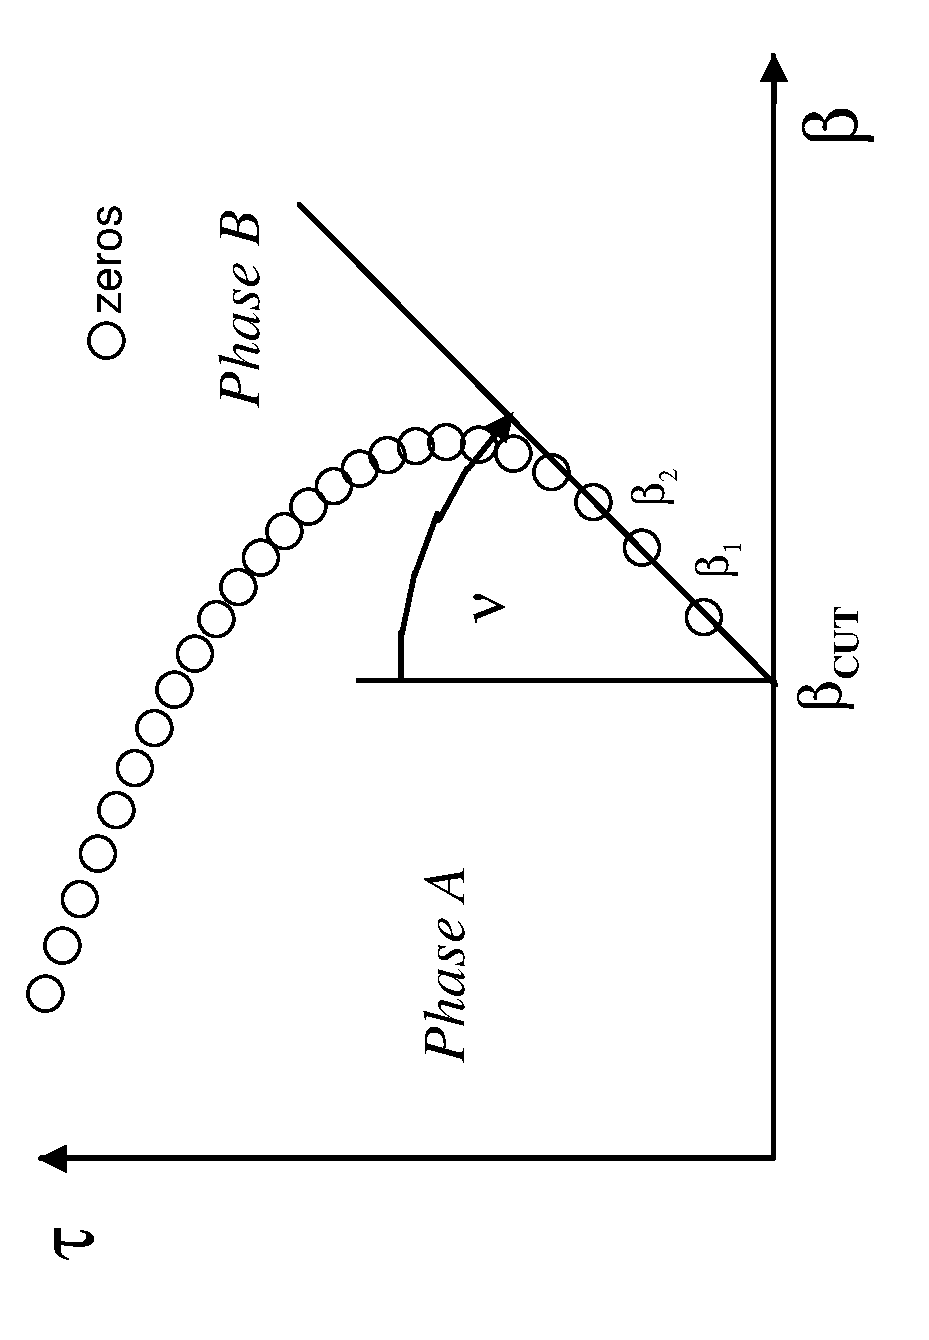
\psfig{file=schematic1.eps,height=3cm,angle=270}}
\caption{Schematic plot of the DOZ illustrating the 
definition of the classification parameters given in the text.}
\label{figure1}
\end{figure}
\begin{figure}
\centerline{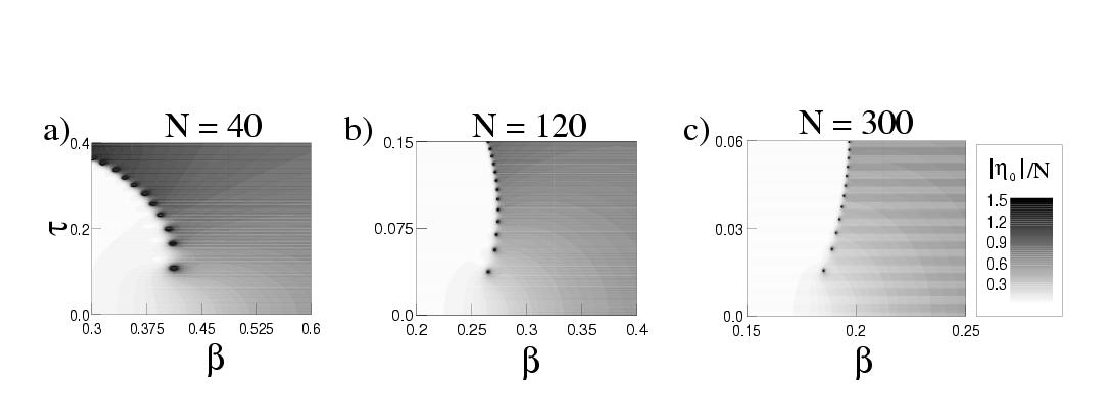
\psfig{file=n0.40-300.cm.bw.ps,width=16cm}}
\caption{Contour plots the ground state
occupation number $\mid \eta_0 \mid /N$ in the complex temperature
plane for 40, 120, and 300 particles in a 3-dimensional isotropic trap.
The black spots indicate the locations of zeros of the partition
function.}
\label{figure2}
\end{figure}
\begin{figure}
\centerline{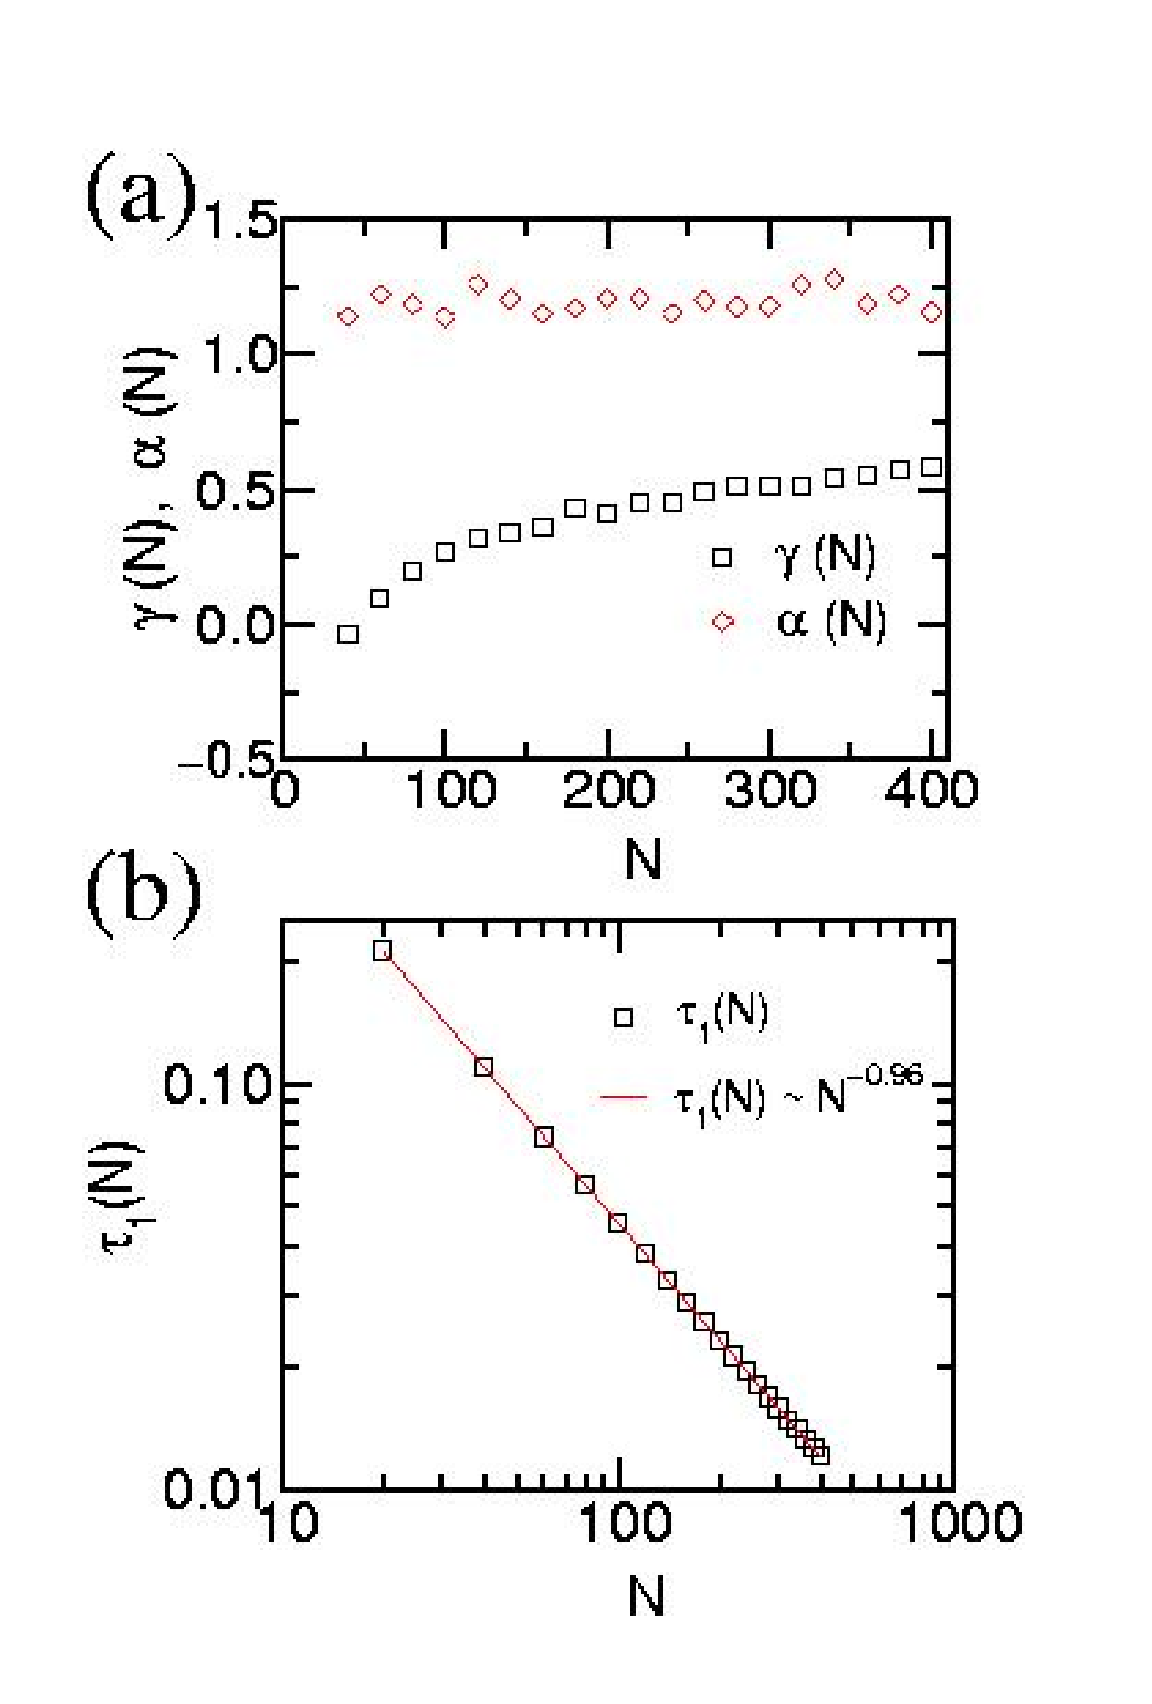
\psfig{file=agt.condmat.eps,width=6cm}}
\caption{Plots of the classification parameters $\alpha$, $\gamma$,
and $\tau_1$ versus the number of particles for a 3-dimensional 
harmonic trap.}
\label{figure3}
\end{figure}
\begin{figure}
\centerline{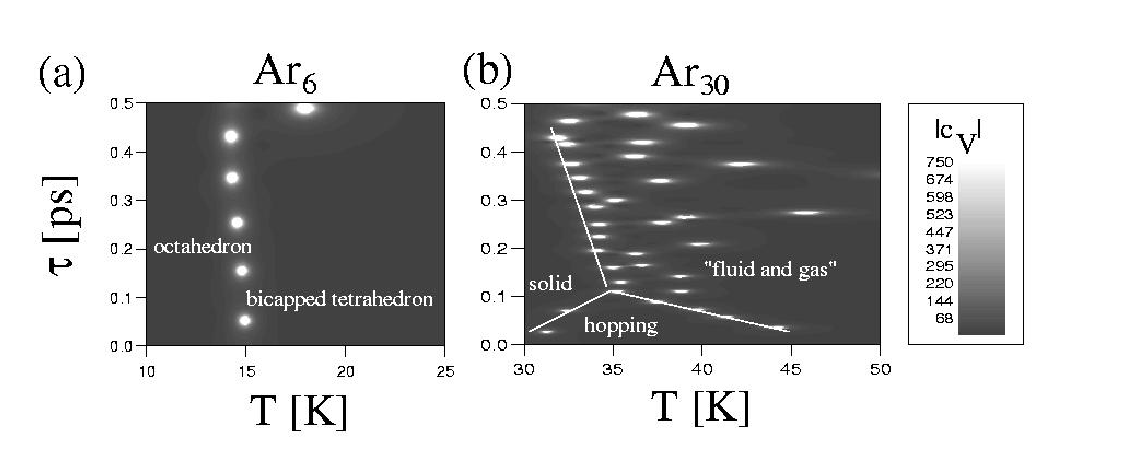
\psfig{file=argon.cm.bw.ps,width=16cm}}
\caption{Contour plots of the specific heat $\mid c_V \mid$ for 
Ar$_6$ and Ar$_{30}$ clusters. }
\label{figure4}
\end{figure}
%
%   Bibliography
%
\begin{thebibliography}{27}

\bibitem{Berry98a}
R. Berry, Nature {\bf 393},  212  (1998).

\bibitem{Schmidt98}
M. Schmidt, B. von Issendorf, and H. Haberland, Nature {\bf 393},  238  (1998).

\bibitem{proykova} A.~Proykova, R.S.~Berry,
        Z.\ Phys.\ {\bf D 40}, 215 (1997). 

\bibitem{mour} O.G.~Mouritsen, {\sl Computer Studies of Phase
    Transitions and Critical Phenomena}, (Springer, Berlin, 1984).

\bibitem{sodium} C.~Ellert, M.~Schmidt, T.~Reiners, H.~Haberland,
        Z.\ Phys. {\bf D 39}, 317 (1997). 

\bibitem{jcptls}
P. Borrmann {\it et~al.}, {\sl to be published in:} J. Chem. Phys.  (1999).

\bibitem{Gross}
D. H. E. Gross, M. E. Madjet, and O. Schapiro, Z. Phys. D {\bf 39}, 75 (1997);
D. H. E. Gross, A. Ecker, and X. Z. Zhang, Annalen Physik {\bf 5}, 446 (1996).

\bibitem{Doye}
D. J. Wales and J. P. K. Doye, J. Chem. Phys. {\bf 103}, 3061 (1995).

\bibitem{Yang1952a}
C.~N. Yang and T. Lee, Phys.\ Rev. {\bf 97},  404  (1952);
C.~N. Yang and T. Lee, Phys.\ Rev. {\bf 87},  410  (1952).

\bibitem{Gross1967}
S. Grossmann and W. Rosenhauer, Z.\ Phys.{\bf 207}, 138 (1967);
S. Grossmann and W. Rosenhauer, Z.\ Phys. {\bf 218}, 437 (1969);
S. Grossmann and V. Lehmann, Z.\ Phys. {\bf 218}, 449 (1969).

\bibitem{extension}
Phase transition with respect to other thermodynamic variables can 
be inspected by making these quantities complex an proceeding in the 
same way as for the temperature.

\bibitem{Titchmarsh}
E. Titchmarsh, {\em The Theory of Functions} (Oxford University Press, Oxford,
  1964).

\bibitem{tasaki:1998}
H. Tasaki, Phys. Rev. Lett. {\bf 80},  1373  (1998).

\bibitem{Anderson1995a}
M.~H. Anderson, J.~R. Ensher, M.~R. Matthews, C.~E. Wieman, and E.~A. Cornell,
Science {\bf 269}, 198 (1995);
C.~C. Bradley, C.~A. Sackett, J.~J. Tollett, and R.~G. Hulet,
Phys. Rev. Lett. {\bf 75}, 1687 (1995);
K.~B. Davis, M.-O. Mewes, M.~R. Andrews, N.~J. van Druten, D.~S. Durfee, D.~M.
Kurn, and W.~Ketterle, Phys. Rev. Lett. {\bf 75}, 3969 (1995).

\bibitem{Bose1924a}
S.~Bose, Z. Phys. {\bf 26}, 178 (1924);
A.~Einstein, Sitzungber. Preuss. Akad. Wiss. {\bf 1925}, 3 (1925).

\bibitem{bose1}
P. Borrmann, G.~Franke, J. Chem. Phys. {\bf 98}, 2484 (1993);
P. Borrmann, J. Harting, O. M{\"u}lken, and E. Hilf, Phys. Rev. A {\bf
  60},  1519  (1999).

\bibitem{Berry:1984a}
R.~S. Berry, J. Jellinek, and N. G., Phys. Rev. A {\bf 30},  919   (1984).

\bibitem{Berry:1984}
R.~S. Berry, J. Jellinek, and G. Natanson, Chem. Phys. Lett. {\bf 107},  227
  (1984).

\bibitem{Beck:1987}
T. Beck, J. Jellinek, and R.~S. Berry, J. Chem. Phys. {\bf 87},  545   (1987).

\bibitem{Jellinek:1986}
J. Jellinek, T.~L. Beck, and R.~S. Berry, J. Chem. Phys. {\bf 84},  2783
  (1986).

\bibitem{Labastie:1990}
P. Labastie and R.~L. Whetten, Phys. Rev. Lett. {\bf 65},  1567   (1990).

\bibitem{Wales:1989}
D.~J. Wales and R.~S. Berry, J. Chem. Phys. {\bf 92},  4283   (1989).

\bibitem{Kunz:1994}
R.~E. Kunz and R.~S. Berry, Phys. Rev. E {\bf 49},  1895   (1994).

\bibitem{bgh96}
P. Borrmann, D. Gloski, and E. Hilf, Surface Review and Letters {\bf 3},  103
  (1996).

\bibitem{hbsh96}
H. Heinze, P. Borrmann, H. Stamerjohanns, and E. Hilf, Z. Phys. {\bf D} {\bf
  40},  190  (1997).

\bibitem{bor94a}
P.~Borrmann, Computational Material Science {\bf 2}, 593 (1994).

\bibitem{Nayak:1995}
S.~K. Nayak, R. Ramaswamy, and C. Chakravarty, Phys. Rev. E {\bf 51},  3376
  (1995).

\bibitem{Ferren:1989}
A.~M. Ferrenberg and R.~H. Swendsen, Phys. Rev. Lett. {\bf 63},  1195  (1989).

\bibitem{fhb93}
G. Franke, E. Hilf, and P. Borrmann, J. Chem. Phys. {\bf 98},  3496  (1993).


\end{thebibliography}
\end{document}
